\subsection{Styrning av svävare}
De olika styralgoritmerna som är implementerade kan väljas om man går in på
"Settings” från huvudprogrammet, som syns i figur \ref{fig:remote}, på
Fjärrkontrollen.
Dessa finns till höger och kan i stort sett ses i figur \ref{fig:remoteApp}. Dessa två avdelningar
populeras dynamiskt beroende på vilka algoritmer som är implementerade.

\begin{figure}[htbp!]
\centering
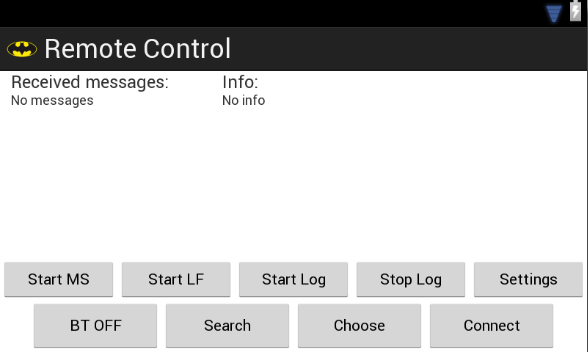
\includegraphics[width=10cm]{../../includes/figures/remote.png}
\caption{Skärmdump av startsidan på Remote.}
\label{fig:remote}
\end{figure}

Ute i huvudprogrammet så startar man lyftfläktarna med hjälp av knappen "Start
LF”. Denna knapp är som en strömbrytare och den byter text till "Stop LF” vid
aktivering av fläktarna.

Styrningen startas med hjälp av knappen "Start
MS”. Denna knapp är som en strömbrytare och den byter text till "Stop MS” vid
aktivering av motorerna.

För att styra svävaren så vickar och vrider operatören på fjärrkontrollen. Ju
större utslag från jämnviktsläget, destå mer kraft levereras till fläktarna och
motorerna.

\begin{figure}[htbp!]
\centering
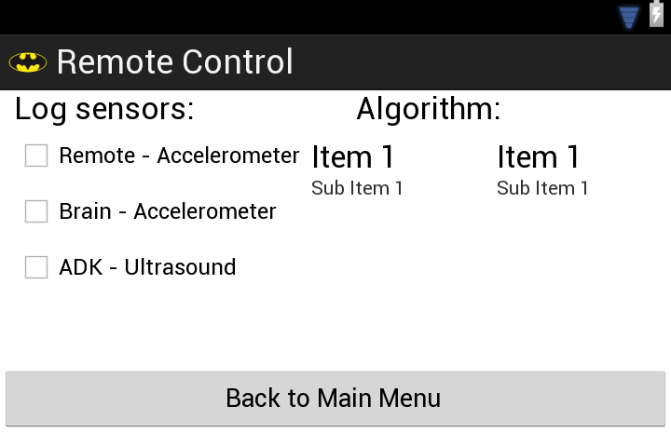
\includegraphics[width=10cm]{../../includes/figures/remote_settings.png}
\caption{Skärmdump av inställningssidan på Remote.}
\label{fig:remoteSettings}
\end{figure}
